\documentclass[%
oneside,                 % oneside: electronic viewing, twoside: printing
final,                   % draft: marks overfull hboxes, figures with paths
10pt]{article}

\listfiles               %  print all files needed to compile this document

\usepackage{relsize,makeidx,color,setspace,amsmath,amsfonts,amssymb}
\usepackage[table]{xcolor}
\usepackage{bm,ltablex,microtype}

\usepackage[pdftex]{graphicx}

\usepackage{fancyvrb} % packages needed for verbatim environments

\usepackage[T1]{fontenc}
%\usepackage[latin1]{inputenc}
\usepackage{ucs}
\usepackage[utf8x]{inputenc}
\usepackage{comment}
\usepackage{listings}
\usepackage{lmodern}
\usepackage{amsmath}        % Latin Modern fonts derived from Computer Modern
\usepackage{float}

% Hyperlinks in PDF:
\definecolor{linkcolor}{rgb}{0,0,0.4}
\usepackage{hyperref}
\hypersetup{
    breaklinks=true,
    colorlinks=true,
    linkcolor=linkcolor,
    urlcolor=linkcolor,
    citecolor=black,
    filecolor=black,
    %filecolor=blue,
    pdfmenubar=true,
    pdftoolbar=true,
    bookmarksdepth=3   % Uncomment (and tweak) for PDF bookmarks with more levels than the TOC
    }
%\hyperbaseurl{}   % hyperlinks are relative to this root

\setcounter{tocdepth}{2}  % levels in table of contents

% --- fancyhdr package for fancy headers ---
\usepackage{fancyhdr}
\fancyhf{} % sets both header and footer to nothing
\renewcommand{\headrulewidth}{0pt}
\fancyfoot[LE,RO]{\thepage}
% Ensure copyright on titlepage (article style) and chapter pages (book style)
\fancypagestyle{plain}{
  \fancyhf{}
  \fancyfoot[C]{{\footnotesize \copyright\ 1999-2018, "Computational Physics I FYS3150/FYS4150":"http://www.uio.no/studier/emner/matnat/fys/FYS3150/index-eng.html". Released under CC Attribution-NonCommercial 4.0 license}}
%  \renewcommand{\footrulewidth}{0mm}
  \renewcommand{\headrulewidth}{0mm}
}
% Ensure copyright on titlepages with \thispagestyle{empty}
\fancypagestyle{empty}{
  \fancyhf{}
  \renewcommand{\footrulewidth}{0mm}
  \renewcommand{\headrulewidth}{0mm}
}

\pagestyle{fancy}


% prevent orhpans and widows
\clubpenalty = 10000
\widowpenalty = 10000

% --- end of standard preamble for documents ---


% insert custom LaTeX commands...

\raggedbottom
\makeindex
\usepackage[totoc]{idxlayout}   % for index in the toc
\usepackage[nottoc]{tocbibind}  % for references/bibliography in the toc

%-------------------- end preamble ----------------------

\usepackage{parskip}
\usepackage{verbatim}

\begin{document}

\newcommand{\exercisesection}[1]{\subsection*{#1}}


\thispagestyle{empty}

\begin{center}
{\LARGE\bf
\begin{spacing}{1.25}
FYS4150/FYS3150 - Project 1
\end{spacing}
}
\end{center}



\begin{center}
\centerline{{\small Ingvild Bergsbak, Oliver Hebnes and Erlend Ousdal}}
\end{center}



\begin{center}
September 10, 2018
\end{center}
% --- end date ---

\vspace{1cm}

\newpage{}


\section{Abstract}

We study the one-dimensional Poisson equation with Dirichlet boundary conditions by rewriting it as a set of linear equations.
The result is verified by comparing it to the exact solution. We find that increasing the number of grid points
will result in a smaller error up until a certain point. We also find that the number of flops in the algorithm is of great significance when computing a large number of grid points, which could be beautifully visualized when measuring CPU time.

\section{Introduction}

This project is our first encounter with the programming language C++ and the subject computational physics. With the one dimensional Poisson equation as a base, we explore the limits of numerical precision and optimization of CPU time.

We will be using C++ for the calculations and Python for plotting our data.

First we look at the general algorithm, and compare it with a specialized one. Thereby we look at the error as a function of step length, and check CPU-time of both algorithms as well as for the LU-decomposition.

The learning curve has been very steep, but it is very motivating getting understandable results.


\section{Theoretical Models and Technicalities}

The purpose of this project is to solve the Poisson equation numerically. We have the equation
\begin{equation*}
-u''(x) = f(x), \hspace{0.5cm} x\in(0,1), \hspace{0.5cm} u(0) = u(1) = 0.
\end{equation*}
and we approximate the second derivative of $u$ by
\begin{equation*}
-u''(x_i)\approx -\frac{v_{i+1}+v_{i-1}-2v_i}{h^2} = f_i  \hspace{0.5cm} \mathrm{for} \hspace{0.1cm} i=1,\dots, n,
\end{equation*}
where $f_i=f(x_i)$.



We define the discretized approximation  to $u$ as $v_i$  with
grid points $x_i=ih$ where $h$ is defined as $h=1/(n+1)$ and $x$ is in the interval from $x_0=0$ to $x_{n+1}=1$.

We have the boundary conditions $v_0 = v_{n+1} = 0$.


Rewriting the approximation gives

\begin{equation*}
-v_{i+1}+2v_{i}-v_{i-1} = h^2f_i=\tilde{b}_i
\end{equation*}


Solving for a slection of $i$ values reveals a pattern\\
\begin{align*}
  i &=1: -v_{2}+2v_{1}-v_0 = -v_{2}+2v_1=\tilde{b}_1\\
  i &=2: -v_{3}+2v_{2}-v_1 = \tilde{b}_2\\
  i &=3: -v_{4}+2v_{3}-v_2 = \tilde{b}_3\\
  \vdots\\
  i &=n: -v_{n+1}+2v_n-v_{n-1} = -v_{n-1}+2v_{n}=\tilde{b}_n\\
\end{align*}

and the equation, $v_{i+1}+v_{i-1}-2v_i =\tilde{b}_i$, can be written as
$$\mathbf{Av}=\mathbf{\tilde{b}} $$\\

where

\begin{equation*}
\mathbf{A}=\begin{bmatrix}
2 & -1 & 0 & \cdots & 0\\
-1 & 2 & -1 & & \\
0 & -1 & 2 & & \vdots \\
\vdots & & & \ddots &-1\\
0 & \cdots & 0 & -1 & 2
\end{bmatrix},
\mathbf{v}=
\begin{bmatrix}
v_1\\
v_2\\
v_3\\
\vdots\\
v_n
\end{bmatrix},
\mathbf{\tilde{b}}=\begin{bmatrix}
\tilde{b}_1\\
\tilde{b}_2\\
\tilde{b}_3\\
\vdots\\
\tilde{b}_n\\
\end{bmatrix}
\end{equation*}

and $\mathbf{A}$ is a $n\times n$ matrix.

\vskip0.7cm
The function $f$ is defined as
$$f(x)=100e^{-10x}$$

Checking the exact solution $u(x)=1-(1-e^{-10})x-e^{-10x}$ by inserting $f$ and $u$ into the Poisson equation.

$$-u''(x)=f(x)$$

\begin{equation*}
\begin{split}
\frac{d^2}{dx^2}u&=\frac{d^2}{dx^2}(1-x+e^{-10}x-e^{-10x})\\
&=\frac{d}{dx}(1+e^{-10}+10e^{-10x})\\
&=-100e^{-10x} = -f(x)
\end{split}
\end{equation*}

Can see that $-u''(x)$ is equal to $f(x)$, and the Poisson equation is satisfied.

\vskip1cm




Gaussian elimination is a very useful method for solving a large set of equations, which can be represented by the form $\mathbf{Av}=\mathbf{b}$. In our case the matrix, $\mathbf{A}$, is a tridigonal matrix, which allows us to simplify the method further.

%---------maybe we dont need the explanation of the tridiag matrix
A tridiagonal matrix is a $n\times n$ matrix with numbers along the diagonal and at the positions directly above and below the diagonal and zeroes on all other positions. To visualize it, the form is shown below.
\begin{equation*}
\mathbf{A}=\begin{bmatrix}
b_1 & c_1 & 0 & \cdots & 0\\
a_1 & b_2 & c_2 & & \\
0 & a_2 & b_3 & & \vdots \\
\vdots & & & \ddots & c_{n-1}\\
0 & \cdots & 0 & a_{n-1} & b_n
\end{bmatrix}
\end{equation*}



First, we use forward substitution, which uses Gaussian elimination to get the matrix on the echolon form, which in this case means $a_i=0$. The Gaussian elimination requires the elements along the diagonal in $\mathbf{A}$ and $\mathbf{\tilde{b}}$ to be updated. The algorithm for this process is given by

\begin{equation*}
\begin{split}
b_i'&=b_i-\frac{a_{i-1}c_{i-1}}{b_{i-1}'}\\
\tilde{b}_i'&=\tilde{b}_i-\frac{a_{i-1}d_{i-1}}{b_{i-1}'}
\end{split}
\end{equation*}

where $b_i'$ and $\tilde{b}_i'$ represent the updated values of $\mathbf{b}$ and $\mathbf{\tilde{b}}$ and $i=1, 2, ..., n$.

Now we are able to solve the equation by backward substitution. This algorithm is given by

\begin{equation*}
\begin{split}
v_n&=b_n'\\
v_i&=\frac{1}{b_i'}(\tilde{b_i}'-c_iv_{i+1})\\
\end{split}
\end{equation*}

where $i=n-1, n-2, ..., 1$.

The theory behind the algorithms for forward and backward substitution are thoroughly described in the lecture notes (Hjort-Jensen, M., 2015 $Computational$ $Physics$), and therefore we will not repeat it in this report.

First we wanted to write a script that would solve the equation $\mathbf{Av}=\mathbf{b}$ for general numbers,
$a_i, b_i$ and $c_i$. We used the matrix $\mathbf A$, but we wrote the algorithm as if the matrix contained random numbers along the diagonals, as shown below.
\begin{lstlisting}
s=a[i-1]/b[i-1]
b[i] = b[i]-s*c[i-1];
b_tilde[i]=b_tilde[i]-s*b_tilde[i-1]
\end{lstlisting}

Later we wanted to specialize our code to the Poisson equation by implementing the additional information we knew about the matrix, which is the fact that $a_i=c_i=-1$ and $b_i=2$ for $i=1, 2, ..., n$. The difference in the algorithm is one line in the forward substitution algorithm, where we define the updated $b_i$ values, which is changed to

\begin{lstlisting}
b[i] = b[0]-1./b[i-1];
\end{lstlisting}
for the special case because we know that $a_i=c_i=-1$ for all $i=1, 2, ..., n$.

When calculating the $v_i$-values, it's interesting to compare the results to the exact values of u(x). This error is calculated as $\epsilon_{i}=log_{10}(|\frac{v_i-u_i}{u_i}1)$. Doing this for a value of n will generate all errors for that n. We can then extract the maximum error value for that specific n. This will be a good way of comparing when n, and thereby h, generates the most exact numerical result.


\newpage{}
\section{Results and Discussion}

The general algorithm has been plotted against the excact value, as seen in figurs 1-3.

\begin{figure}[H]
  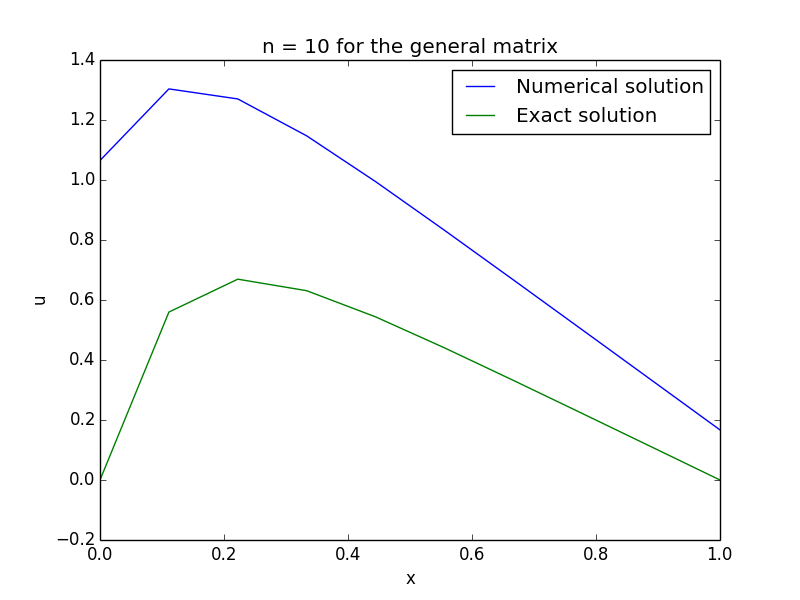
\includegraphics[scale=0.5]{figur1b_10.png}
  \centering
  \caption{Matrix with the size of 10 x 10 compared to the closed-form solution.}
  \label{1b_10}
\end{figure}
\begin{figure}[H]
  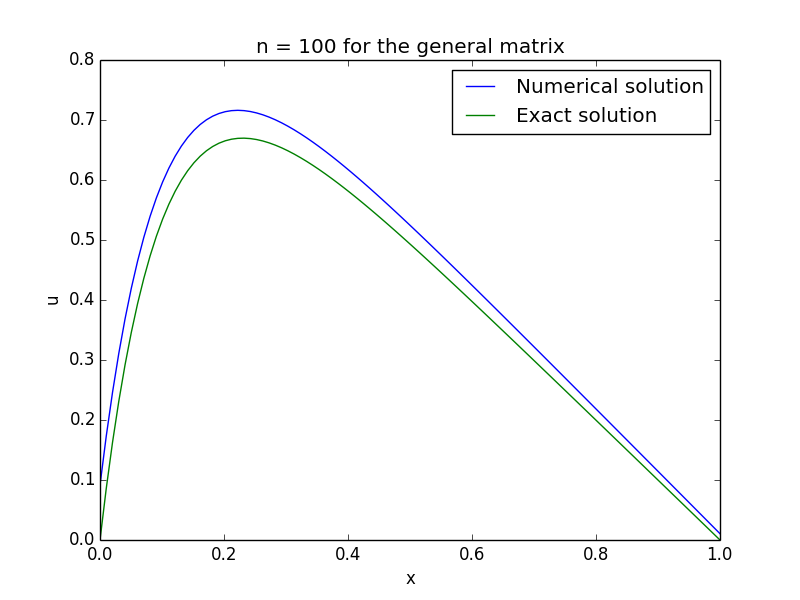
\includegraphics[scale=0.5]{figur1b_100.png}
  \caption{Matrix with the size of 100 x 100 compared to the closed-form solution.}
  \label{1b_100}
\end{figure}



\begin{figure}[H]
  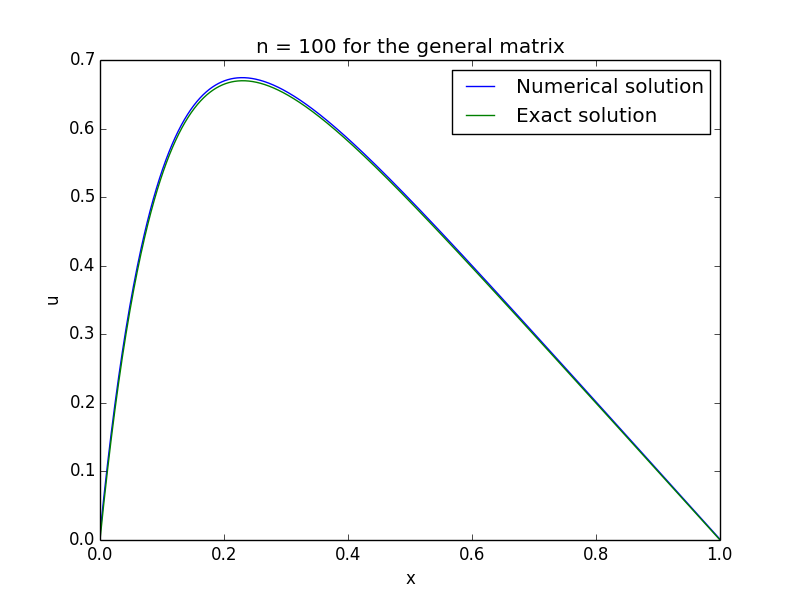
\includegraphics[scale=0.5]{figur1b_1000.png}
  \caption{Matrix with the size of 1000 x 1000 compared to the closed-form solution.}
  \label{1b_1000}
\end{figure}
\newpage{}

From figure 1-3 it is pretty obvious that increasing the number of grid points makes the error decrease. The step length between each $v$ value is decided by $h$, which is inversely proportional to $n$. This means that a bigger $n$ gives a smaller step length. The smaller the step length, the more accurate the numerical approximation will be, until $h$ reaches a minimum value. When this happens, the error will increase. This is plotted logarithmically in figure 4.

\begin{figure}[H]
  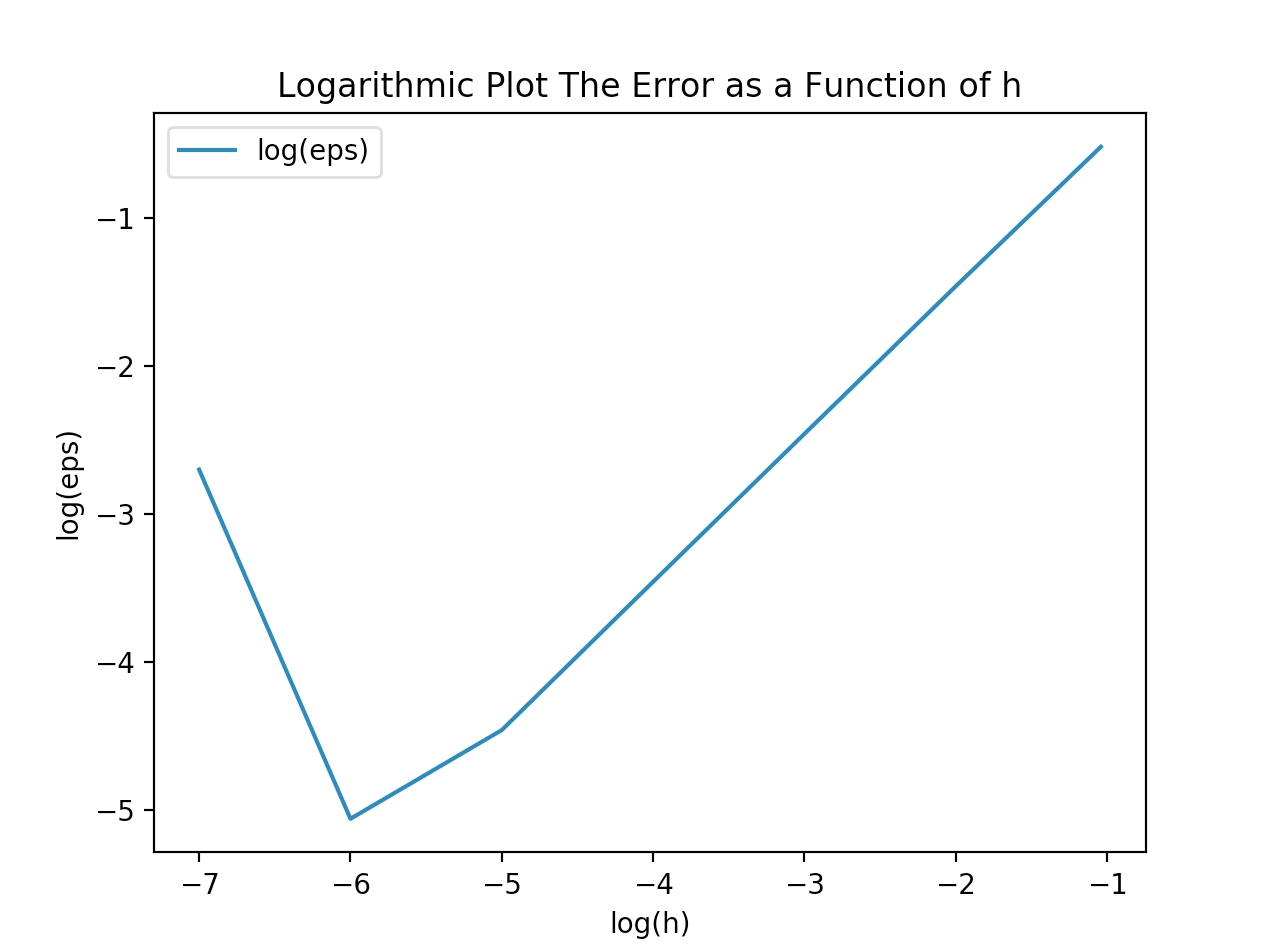
\includegraphics[scale=0.5]{fig-error.png}
  \caption{$log_{10}(eps_n)$ vs $log_{10}(h)$}
  \label{1d}
\end{figure}

As we can see from figure 4, the most exact result will be for a $10^6*10^6$ matrix. When n=$10^7$, the error increases again. This is because for each iteration we get a round off error, which is about $10^{-7}$, and when the step size is of the same order or lower, the round off error will become significant, and numerical precision will decrease.


We check the efficiency of the general and the specific algorithm by running the c++ code while timing the algorithm for $n=10^6$. We check each algorithm ten times each and then find the average time of both of them. The result is that the specific time uses 0.07571 seconds while the general uses 0.079627 seconds. This means that the specific algorithm is faster.
This makes sense because the number of flops from the general algorithm scales with $8N$ ($5N$ flops from the forward substitution, and $3N$ flops from the backward substitution), and the flops from the specific case scales with $7N$ ($4N$ flops from the forward substitution, and $3N$ flops from the backward substitution).

When comparing the LU decomposition algorithm against our specialized algorithm, we look at the elapsed time of the algorithms with $n=10$, $n=100$ and $n=1000$. We run the algorithms ten times each and then compute the average value. The results can be found in table 1 and table 2.
The flops in LU-decomposition scales as $\frac{2}{3} n^3$. If we are going to use LU-decomposition for computing the a $10^5$ x $10^5$ matrix, it requires $\frac{2}{3}10^{15}$ flops. This requires an tremendous amount more memory compared to our general and special logarithm.

\begin{table}[H]
    \centering
    \begin{tabular}{|l|c|c|r|}
    \hline
     run & n=10 & n=100 & n=1000\\
     \hline
      1  & 0.000111 s & 0.000183 s & 0.012385 s\\
      2  & 0.000104 s & 0.000166 s & 0.01338 s\\
      3  & 0.000103 s & 0.000171 s & 0.009844 s\\
      4  & 0.000108 s & 0.000151 s & 0.009508 s\\
      5  & 0.000123 s & 0.000187 s & 0.009331 s\\
      6  & 0.000126 s & 0.000175 s & 0.013402 s\\
      7  & 0.000103 s & 0.000152 s & 0.012531 s\\
      8  & 0.000105 s & 0.000153 s & 0.010998 s\\
      9  & 0.000104 s & 0.000162 s & 0.008004 s\\
      10 & 0.000104 s & 0.000156 s & 0.010687 s\\
      \hline
      Average & 0.000109 s & 0.000166 s & 0.011007 s\\
      \hline
    \end{tabular}
    \caption{Elapsed time for LU decomposition in c++ for n=10, n=100 and n=1000.}
    \label{tab:my_label}
\end{table}

\begin{table}[H]
    \centering
    \begin{tabular}{|l|c|c|r|}
    \hline
     run & n=10 & n=100 & n=1000\\
     \hline
      1  & $9.0*10^{-6}$ s & $1.7*10^{-5}$ s & 0.000155 s\\
      2  & $9.0*10^{-6}$ s & $1.7*10^{-5}$ s & 0.000111 s\\
      3  & $6.0*10^{-6}$ s & $2.2*10^{-5}$ s & $0.000076$ s\\
      4  & $9.0*10^{-6}$ s& $1.7*10^{-5}$ s & 0.000109 s\\
      5  & $5.0*10^{-6}$ s& $2.2*10^{-5}$ s & 0.000111 s\\
      6  & $6.0*10^{-6}$ s& $1.7*10^{-5}$ s  & 0.000108 s\\
      7  & $7.0*10^{-6}$ s & $2.2*10^{-5}$ s & 0.000158 s\\
      8  & $7.0*10^{-6}$ s & $2.3*10^{-5}$ s & 0.000151 s\\
      9  & $7.0*10^{-6}$ s & $2.3*10^{-5}$ s  & 0.000155 s\\
      10 & $9.0*10^{-6}$ s & $2.2*10^{-5}$ s & 0.000109 s\\
      \hline
      Average & $7.4*10^{-6}$ s & $2.02*10^{-5}$ s & $1.203*10^{-4}$ s\\
      \hline
    \end{tabular}
    \caption{Elapsed time for the specialized in c++ for n=10, n=100 and n=1000.}
    \label{tab:my_label}
\end{table}

As we can see, our specialized algorithm is a lot faster than the LU decomposition, which makes sense because of the number of flops.


\section{Conclusion and Perspective}

From our results it's easy to see that the specialized algorithm is the most flop-efficient of the three computed ones. LU-decomposition is extremely easy to use, and is therefore beautiful in its own way when dealing with small matrices. However the flop count is way too high when facing matrices of high magnitude.

We found that C++ was a valuable tool when computing algorithm, but Python excelled in presenting visual data. This is why we implemented them both in our project. This will sure get handy when diving into the deep pool of Computational Physics.

Github got implemented in our project a bit late which makes the version control go back to the beginning. For our next project we will enjoy the pleasure of git and GitHub from the very start.

Finally we also found that being structured and planning an effective code requires a bit of work, especially when dealing with dynamic memory allocations. 

\section{Appendix}

-Link to our GitHub repository:
https://github.com/ohebbi/compphys.git

\section{Bibliography}

- Hjort-Jensen, M., 2015 $Computational$ $physics$, accesible at course github repository. 551 pages.





\end{document}





\begin{equation*}

\end{equation*}
